\documentclass[a4paper]{article}
\usepackage[utf8]{inputenc}
\usepackage[spanish, es-tabla, es-noshorthands]{babel}
\usepackage[table,xcdraw]{xcolor}
\usepackage[a4paper, footnotesep = 1cm, width=20cm, top=2.5cm, height=25cm, textwidth=18cm, textheight=25cm]{geometry}
%\geometry{showframe}

\usepackage{tikz}
\usepackage{amsmath}
\usepackage{amsfonts}
\usepackage{amssymb}
\usepackage{float}
\usepackage{graphicx}
\usepackage{caption}
\usepackage{subcaption}
\usepackage{multicol}
\usepackage{multirow}
\setlength{\doublerulesep}{\arrayrulewidth}
\usepackage{booktabs}
\usepackage{mathrsfs,amsmath}
\usepackage{hyperref}
\hypersetup{
    colorlinks=true,
    linkcolor=blue,
    filecolor=magenta,      
    urlcolor=blue,
    citecolor=blue,    
}

\newcommand{\quotes}[1]{``#1''}
\usepackage{array}
\newcolumntype{C}[1]{>{\centering\let\newline\\\arraybackslash\hspace{0pt}}m{#1}}
\usepackage[american]{circuitikz}
\usetikzlibrary{calc}
\usepackage{fancyhdr}
\usepackage{units} 

\graphicspath{./Imagenes}

\pagestyle{fancy}
\fancyhf{}
\lhead{22.05 ASSD}
\rhead{Mechoulam, Lambertucci, Rodriguez, Londero}
\rfoot{Página \thepage}

\begin{document}
\section{Entorno de simulación}
La GUI fue desarrollada con la herramiente GNU Radio, la cual es similar a simulink de matlab, permitiendo realizar simulaciones de signal prossesing en tiempo real, este fue desarrollado en C++ y python.
Siendo (\ref{fig:gnu}) la interfaz del programa,
 \begin{figure}[H]
	\centering
	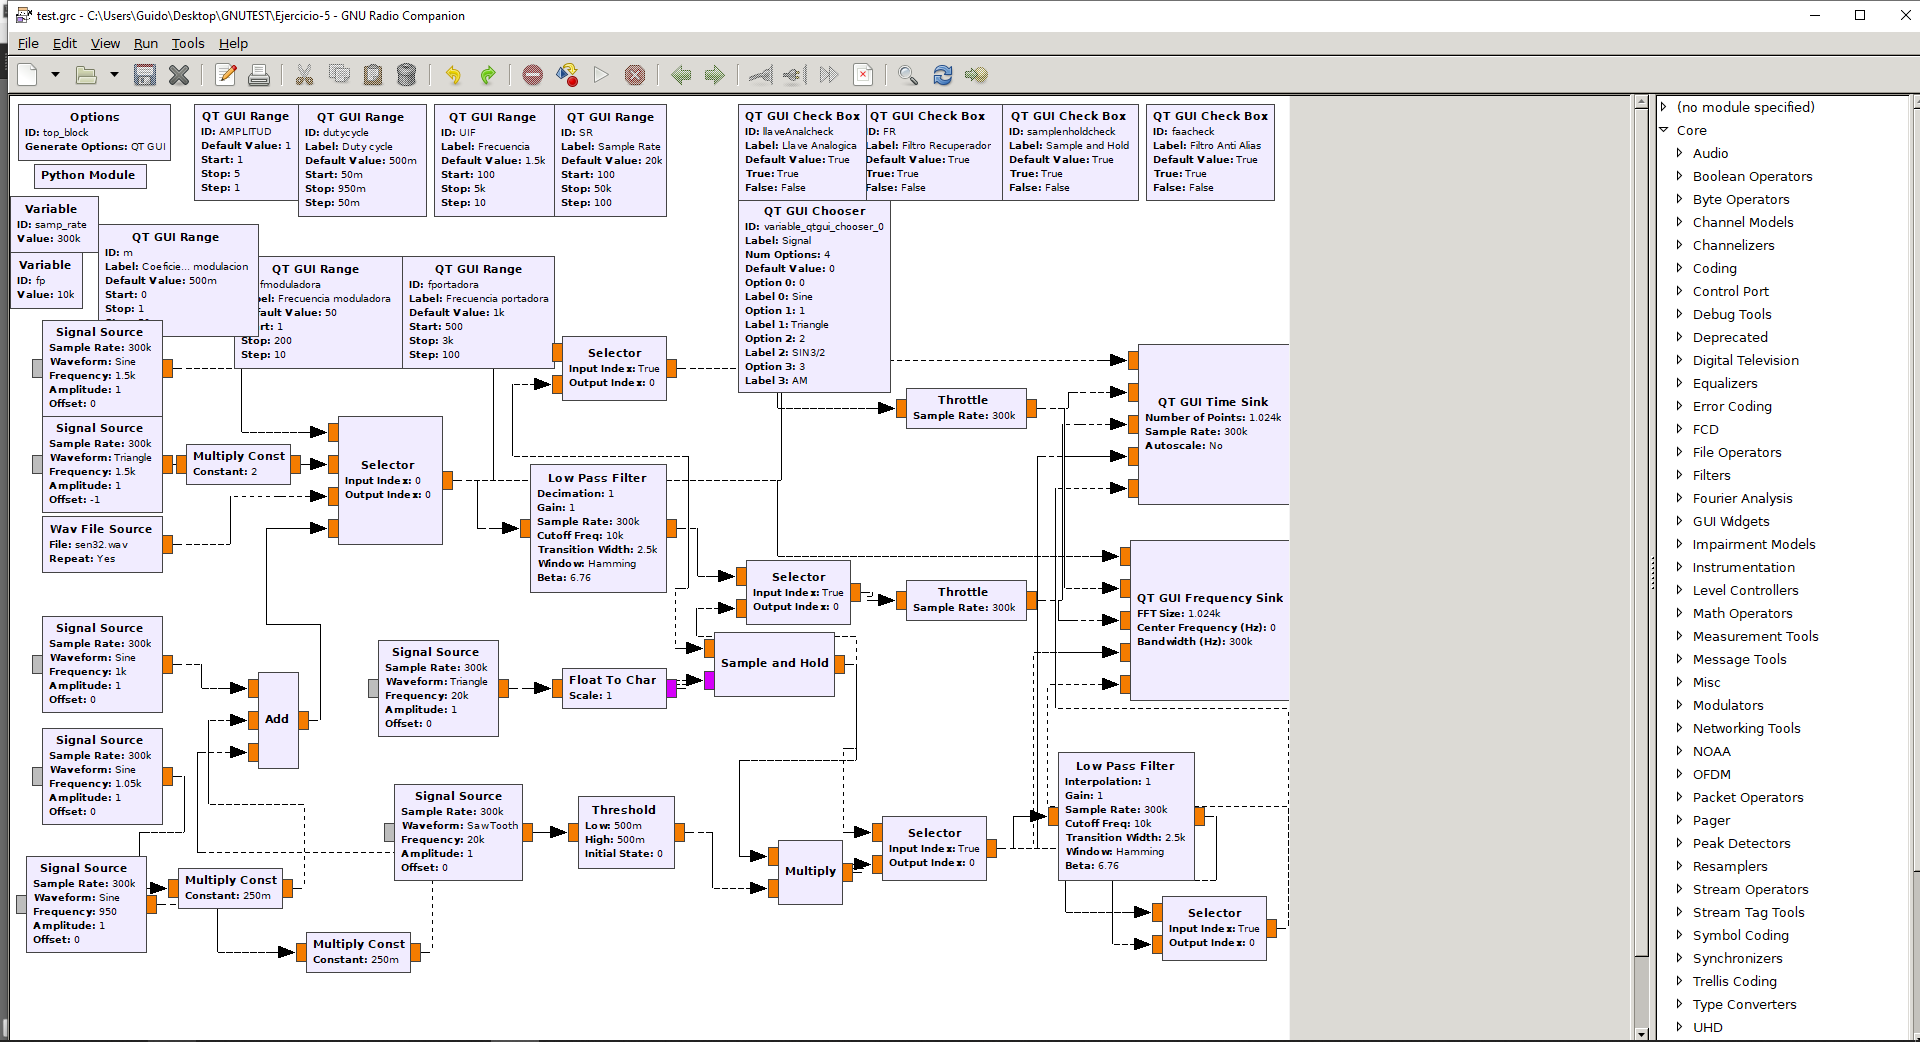
\includegraphics[width=0.9\textwidth]{ImagenesEjercicio5/gnuradio.PNG}
\caption{Interfaz GNURadio.}
	\label{fig:gnu}
\end{figure}
Para correr el programa lo primero es descargar el software desde la \href{http://www.gcndevelopment.com/gnuradio/downloads.htm}{página}, luego debe abrirse la aplicación "GNURadio companion", la cual abre el entorno de simulación, luego se le debe dar al simbolo de play para comenzar.Se le debe abrir la siguiente interfaz.
 \begin{figure}[H]
	\centering
	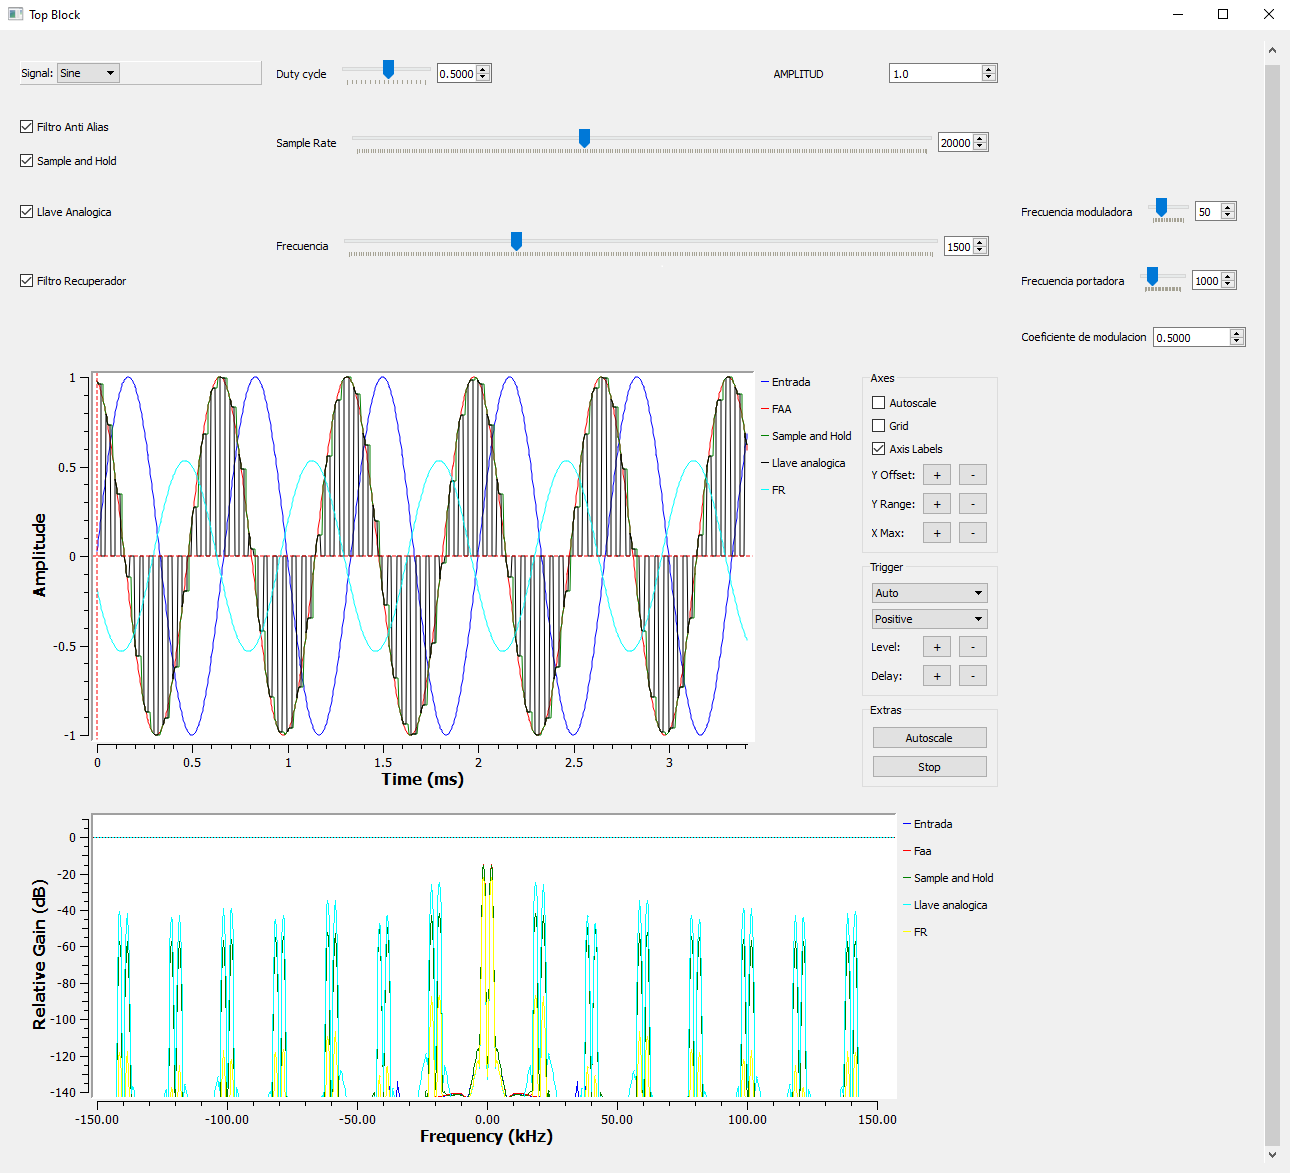
\includegraphics[width=0.9\textwidth]{ImagenesEjercicio5/gui.PNG}
\caption{GUI.}
	\label{fig:GUI}
\end{figure}
\footnote{A veces no se refresca bien la señal triangular, para que se actualize cambie la amplitud.}
\end{document}